% ML4PS @ NeurIPS workshop paper — 4-page limit (excl. references).
% Style: official neurips_2025.sty (vendored). TODO: swap for the ML4PS 2026
% template when released; until then the footer is set manually below.
\documentclass{article}
\usepackage[final]{neurips_2025}

\usepackage[utf8]{inputenc}
\usepackage[T1]{fontenc}
\usepackage{hyperref}
\usepackage{url}
\usepackage{booktabs}
\usepackage{amsfonts}
\usepackage{microtype}
\usepackage{graphicx}
\usepackage{xcolor}
\usepackage{tikz}
\usetikzlibrary{arrows.meta, positioning}

% --- ML4PS workshop footer (replaces the NeurIPS notice line) ---
\makeatletter
\renewcommand{\@noticestring}{%
  Machine Learning and the Physical Sciences Workshop, NeurIPS 2026.\ % TODO: confirm exact ML4PS 2026 footer wording
}
\makeatother

\newcommand{\todo}[1]{\textcolor{red}{[TODO: #1]}}

\title{An LLM-Driven Closed-Loop AI Scientist for Dark-Matter Substructure
Classification in Strong Gravitational Lensing}
% TODO: title is a working draft — refine with co-authors.

\author{%
  Aatmaj Amol Salunke\\
  Northeastern University\\
  \texttt{\todo{email}}\\
  \And
  Pranath Reddy\\
  University of Florida\\
  \texttt{\todo{email}}\\
  \And
  Michael W.\ Toomey\\
  Massachusetts Institute of Technology\\
  \texttt{\todo{email}}\\
  \And
  Sergei Gleyzer\\
  University of Alabama\\
  \texttt{\todo{email}}\\
}

\begin{document}

\maketitle

\begin{abstract}
\todo{150--200 words. What goes here: (1) motivation — autonomous ML
experimentation for lensing substructure; (2) the system — a typed multi-agent
pipeline with an LLM planner that closes the loop (observe metrics $\to$ one typed
change $\to$ retrain), plus a tree-based architecture search with an LLM judge;
(3) headline results — planner closes a 0.23 train/val gap in one intervention
(+5.0 val pts); full search+tune runs end-to-end in $\sim$6 min on a laptop;
(4) honesty clause — prototype, single-seed, limitations stated.}
\end{abstract}

\section{Introduction}
\todo{2--3 paragraphs. Dark-matter substructure classification in strong lensing
(cite DeepLense papers \citep{alexander2020deep,alexander2021decoding,toomey2022deep});
the cost of manual ML experimentation; LLM agents as experimenters — ReAct
\citep{yao2023react}, LLM-as-judge \citep{zheng2023judging}; our contribution: a
typed, bias-controlled closed loop that demonstrably fixes overfitting on real
simulated lensing data, and an honest account of where LLM-driven search helps and
where it does not (yet).}

\section{The AI-Scientist Pipeline}
\label{sec:pipeline}
\todo{Describe Figure~\ref{fig:pipeline}: agents (simulate, design, train, infer,
analyze, plan) exchanging typed Pydantic contracts; the ReAct planner (metrics-only
observations, one typed change per iteration, code-side stop guards, swappable
strategy protocol); the tree search (generate $\sim$10 buildable candidates, LLM
judge top-4, short real training, code-side pruning, one refinement round); bias
controls in prompts (no preferred-architecture hints). Note payload discipline:
prediction arrays never pass through the LLM context.}

\begin{figure}[t]
  \centering
  % TODO: replace this TikZ stub with the real pipeline figure
  % (figures/pipeline.pdf) before submission.
  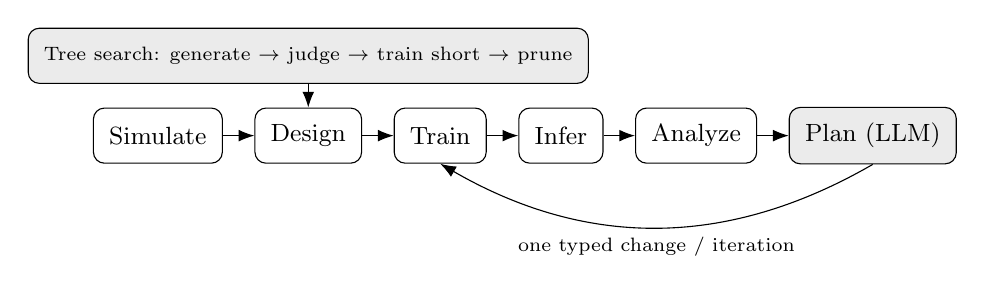
\begin{tikzpicture}[
      node distance=3mm and 4mm,
      stage/.style={draw, rounded corners, minimum height=7mm, inner sep=2mm, font=\small},
      arr/.style={-{Latex[length=2mm]}}
    ]
    \node[stage] (sim) {Simulate};
    \node[stage, right=of sim] (design) {Design};
    \node[stage, right=of design] (train) {Train};
    \node[stage, right=of train] (infer) {Infer};
    \node[stage, right=of infer] (analyze) {Analyze};
    \node[stage, right=of analyze, fill=black!8] (plan) {Plan (LLM)};
    \draw[arr] (sim) -- (design);
    \draw[arr] (design) -- (train);
    \draw[arr] (train) -- (infer);
    \draw[arr] (infer) -- (analyze);
    \draw[arr] (analyze) -- (plan);
    \draw[arr] (plan.south) to[out=-150, in=-30] node[below, font=\scriptsize]
      {one typed change / iteration} (train.south);
    \node[stage, above=of design, fill=black!8, font=\scriptsize]
      (search) {Tree search: generate $\to$ judge $\to$ train short $\to$ prune};
    \draw[arr] (search) -- (design);
  \end{tikzpicture}
  \caption{\todo{Final caption.} The closed-loop pipeline: typed agent contracts,
  the ReAct planner, and the tree-based architecture search feeding the tuner.}
  \label{fig:pipeline}
\end{figure}

\section{Experimental Setup}
\label{sec:setup}
\todo{Dataset: 9{,}000 self-generated Model\_I images (3{,}000/class: no\_sub, cdm,
axion; 150$\times$150, single channel) using the DeepLenseSim recipe with
lenstronomy 1.9.2 \citep{birrer2018lenstronomy} and pyHalo \citep{gilman2020pyhalo}
— explicitly NOT the official released dataset. 7{,}200/1{,}800 train/val split;
closed-loop experiments use a 1{,}800-image training subset. Training: from-scratch
ResNets/CNNs \citep{he2016deep}, AdamW \citep{loshchilov2019adamw}, seeded, Apple
M-series (MPS), torch 2.13. LLMs: gpt-5.6-luna (search+combined run) and gpt-5.2
(planner-only run); temperature provider-default (unpinned). State limitations:
single seed, no separate test set (val used for both selection and reporting).}

\section{Results and Discussion}
\label{sec:results}
\todo{Walk Tables~\ref{tab:planner},~\ref{tab:final}: (1) the planner correctly
diagnoses overfitting from metrics alone and closes the gap in one intervention;
(2) full-data baseline numbers; (3) the combined search+tune run (winner
cnn\_medium\_multistage, 0.29M params; tuned val 0.749) does NOT yet beat the
planner-tuned resnet34 (0.802) — discuss low-fidelity evaluation bias and the two
ablation findings (4-epoch noise; task-wording bias). Runtime: 5.9 min end-to-end
on a laptop; $\sim$4$\times$ estimated for the full dataset.}

\begin{table}[t]
  \caption{Closed-loop planner trajectory on the 1{,}800-image subset (seeded;
  planner = gpt-5.2). One planner intervention closes the train/val gap and
  improves validation accuracy by 5.0 points.}
  \label{tab:planner}
  \centering
  \small
  \begin{tabular}{llccccc}
    \toprule
    It. & Configuration & Train & Val & Gap & AUC & Planner decision \\
    \midrule
    0 & resnet34, no regularization, 25 ep & 0.9839 & 0.7517 & 0.2322 & 0.8922 &
      augment + early stopping \\
    1 & + augmentation + early stopping & 0.7926 & \textbf{0.8017} &
      \textbf{$-$0.0091} & \textbf{0.9187} & stop (gap closed) \\
    \bottomrule
  \end{tabular}
\end{table}

\begin{table}[t]
  \caption{Full-dataset baseline (7{,}200 train / 1{,}800 val): resnet34 chosen by
  the model-design agent, 30 epochs. Errors concentrate in cdm vs.\ axion — the
  physically hard substructure-type distinction.}
  \label{tab:final}
  \centering
  \small
  \begin{tabular}{lcccc}
    \toprule
    Class & Precision & Recall & F1 & $n$ \\
    \midrule
    no\_sub & 0.956 & 0.933 & 0.944 & 600 \\
    cdm     & 0.755 & 0.762 & 0.758 & 600 \\
    axion   & 0.803 & 0.815 & 0.809 & 600 \\
    \midrule
    \multicolumn{5}{l}{Overall: accuracy 0.8367, macro AUC 0.9429.} \\
    \bottomrule
  \end{tabular}
\end{table}

\section{Conclusion}
\todo{3--4 sentences: typed closed-loop AI scientist works end to end on real
simulated lensing data and fixes a concrete pathology (overfitting) autonomously;
architecture search adds automation, with evaluation fidelity as the key open knob;
next steps — multi-seed runs, held-out test split, higher-fidelity candidate
evaluation, and letting the loop revisit architecture.}

\begin{ack}
\todo{Match last year's ML4PS/DeepLense acknowledgement wording.} This work was
supported by Google Summer of Code 2026 with the Machine Learning for Science
(ML4SCI) organization.
\end{ack}

\bibliographystyle{plainnat}
\bibliography{references}

\end{document}
